% AUTO-GENERATED by code/figlib.py helpers -- do not edit
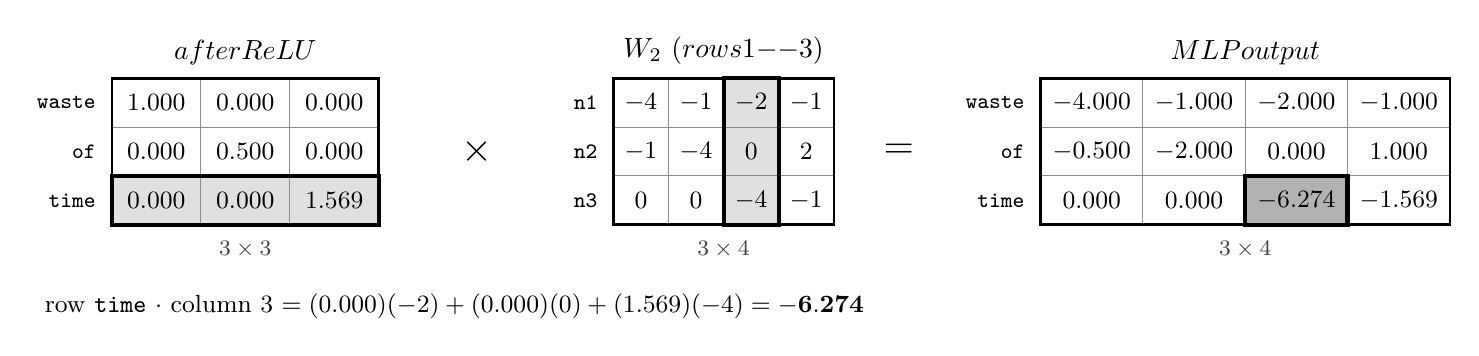
\begin{tikzpicture}
\draw[black!45, fill=white] (0.975,0.930) rectangle (2.105,0.310);
\node[font=\small, text=black] at (1.540,0.620) {$1.000$};
\draw[black!45, fill=white] (2.105,0.930) rectangle (3.235,0.310);
\node[font=\small, text=black] at (2.670,0.620) {$0.000$};
\draw[black!45, fill=white] (3.235,0.930) rectangle (4.365,0.310);
\node[font=\small, text=black] at (3.800,0.620) {$0.000$};
\draw[black!45, fill=white] (0.975,0.310) rectangle (2.105,-0.310);
\node[font=\small, text=black] at (1.540,-0.000) {$0.000$};
\draw[black!45, fill=white] (2.105,0.310) rectangle (3.235,-0.310);
\node[font=\small, text=black] at (2.670,-0.000) {$0.500$};
\draw[black!45, fill=white] (3.235,0.310) rectangle (4.365,-0.310);
\node[font=\small, text=black] at (3.800,-0.000) {$0.000$};
\draw[black!45, fill=black!12] (0.975,-0.310) rectangle (2.105,-0.930);
\node[font=\small, text=black] at (1.540,-0.620) {$0.000$};
\draw[black!45, fill=black!12] (2.105,-0.310) rectangle (3.235,-0.930);
\node[font=\small, text=black] at (2.670,-0.620) {$0.000$};
\draw[black!45, fill=black!12] (3.235,-0.310) rectangle (4.365,-0.930);
\node[font=\small, text=black] at (3.800,-0.620) {$1.569$};
\draw[line width=1.4pt] (0.975,-0.310) rectangle (4.365,-0.930);
\draw[line width=0.9pt] (0.975,0.930) rectangle (4.365,-0.930);
\node[anchor=east, font=\footnotesize\ttfamily] at (0.895,0.620) {waste};
\node[anchor=east, font=\footnotesize\ttfamily] at (0.895,-0.000) {of};
\node[anchor=east, font=\footnotesize\ttfamily] at (0.895,-0.620) {time};
\node[anchor=south, font=\normalsize] at (2.670,0.980) {$\text{after ReLU}$};
\node[anchor=north, font=\footnotesize, text=black!75] at (2.670,-1.010) {$3\times3$};
\node[font=\Large] at (5.615,0) {$\times$};
\draw[black!45, fill=white] (7.345,0.930) rectangle (8.045,0.310);
\node[font=\small, text=black] at (7.695,0.620) {$-4$};
\draw[black!45, fill=white] (8.045,0.930) rectangle (8.745,0.310);
\node[font=\small, text=black] at (8.395,0.620) {$-1$};
\draw[black!45, fill=black!12] (8.745,0.930) rectangle (9.445,0.310);
\node[font=\small, text=black] at (9.095,0.620) {$-2$};
\draw[black!45, fill=white] (9.445,0.930) rectangle (10.145,0.310);
\node[font=\small, text=black] at (9.795,0.620) {$-1$};
\draw[black!45, fill=white] (7.345,0.310) rectangle (8.045,-0.310);
\node[font=\small, text=black] at (7.695,-0.000) {$-1$};
\draw[black!45, fill=white] (8.045,0.310) rectangle (8.745,-0.310);
\node[font=\small, text=black] at (8.395,-0.000) {$-4$};
\draw[black!45, fill=black!12] (8.745,0.310) rectangle (9.445,-0.310);
\node[font=\small, text=black] at (9.095,-0.000) {$0$};
\draw[black!45, fill=white] (9.445,0.310) rectangle (10.145,-0.310);
\node[font=\small, text=black] at (9.795,-0.000) {$2$};
\draw[black!45, fill=white] (7.345,-0.310) rectangle (8.045,-0.930);
\node[font=\small, text=black] at (7.695,-0.620) {$0$};
\draw[black!45, fill=white] (8.045,-0.310) rectangle (8.745,-0.930);
\node[font=\small, text=black] at (8.395,-0.620) {$0$};
\draw[black!45, fill=black!12] (8.745,-0.310) rectangle (9.445,-0.930);
\node[font=\small, text=black] at (9.095,-0.620) {$-4$};
\draw[black!45, fill=white] (9.445,-0.310) rectangle (10.145,-0.930);
\node[font=\small, text=black] at (9.795,-0.620) {$-1$};
\draw[line width=1.4pt] (8.745,0.930) rectangle (9.445,-0.930);
\draw[line width=0.9pt] (7.345,0.930) rectangle (10.145,-0.930);
\node[anchor=east, font=\footnotesize\ttfamily] at (7.265,0.620) {n1};
\node[anchor=east, font=\footnotesize\ttfamily] at (7.265,-0.000) {n2};
\node[anchor=east, font=\footnotesize\ttfamily] at (7.265,-0.620) {n3};
\node[anchor=south, font=\normalsize] at (8.745,0.980) {$W_2\ (\text{rows }1\text{--}3)$};
\node[anchor=north, font=\footnotesize, text=black!75] at (8.745,-1.010) {$3\times4$};
\node[font=\Large] at (10.970,0) {$=$};
\draw[black!45, fill=white] (12.770,0.930) rectangle (14.070,0.310);
\node[font=\small, text=black] at (13.420,0.620) {$-4.000$};
\draw[black!45, fill=white] (14.070,0.930) rectangle (15.370,0.310);
\node[font=\small, text=black] at (14.720,0.620) {$-1.000$};
\draw[black!45, fill=white] (15.370,0.930) rectangle (16.670,0.310);
\node[font=\small, text=black] at (16.020,0.620) {$-2.000$};
\draw[black!45, fill=white] (16.670,0.930) rectangle (17.970,0.310);
\node[font=\small, text=black] at (17.320,0.620) {$-1.000$};
\draw[black!45, fill=white] (12.770,0.310) rectangle (14.070,-0.310);
\node[font=\small, text=black] at (13.420,-0.000) {$-0.500$};
\draw[black!45, fill=white] (14.070,0.310) rectangle (15.370,-0.310);
\node[font=\small, text=black] at (14.720,-0.000) {$-2.000$};
\draw[black!45, fill=white] (15.370,0.310) rectangle (16.670,-0.310);
\node[font=\small, text=black] at (16.020,-0.000) {$0.000$};
\draw[black!45, fill=white] (16.670,0.310) rectangle (17.970,-0.310);
\node[font=\small, text=black] at (17.320,-0.000) {$1.000$};
\draw[black!45, fill=white] (12.770,-0.310) rectangle (14.070,-0.930);
\node[font=\small, text=black] at (13.420,-0.620) {$0.000$};
\draw[black!45, fill=white] (14.070,-0.310) rectangle (15.370,-0.930);
\node[font=\small, text=black] at (14.720,-0.620) {$0.000$};
\draw[black!45, fill=black!30] (15.370,-0.310) rectangle (16.670,-0.930);
\node[font=\small, text=black] at (16.020,-0.620) {$-6.274$};
\draw[black!45, fill=white] (16.670,-0.310) rectangle (17.970,-0.930);
\node[font=\small, text=black] at (17.320,-0.620) {$-1.569$};
\draw[line width=1.6pt] (15.370,-0.310) rectangle (16.670,-0.930);
\draw[line width=0.9pt] (12.770,0.930) rectangle (17.970,-0.930);
\node[anchor=east, font=\footnotesize\ttfamily] at (12.690,0.620) {waste};
\node[anchor=east, font=\footnotesize\ttfamily] at (12.690,-0.000) {of};
\node[anchor=east, font=\footnotesize\ttfamily] at (12.690,-0.620) {time};
\node[anchor=south, font=\normalsize] at (15.370,0.980) {$\text{MLP output}$};
\node[anchor=north, font=\footnotesize, text=black!75] at (15.370,-1.010) {$3\times4$};
\node[anchor=north west, font=\small, align=left] at (0,-1.680) {row \texttt{time} $\cdot$ column 3 $= (0.000)(-2) + (0.000)(0) + (1.569)(-4) = \mathbf{-6.274}$};
\end{tikzpicture}
